\documentclass[a4paper, 11pt]{article}
\usepackage{comment} % enables the use of multi-line comments (\ifx \fi) 
\usepackage{lipsum} %This package just generates Lorem Ipsum filler text. 
\usepackage{fullpage} % changes the margin
\usepackage{graphicx}
\usepackage{color}
\graphicspath{ {./images/} }

\begin{document}
%Header-Make sure you update this information!!!!

\noindent
\large\textbf{Tema de cas\u{a}} \hfill \textbf{Programarea Aplica\c{t}iilor \^{i}n Timp Real} \\
\normalsize Echipa: B\u{a}lan Mihai, Ciobanu \c{S}tefan, Sp\^{i}nu Andrei  \hfill Sem. 2, 2021-2022 \\ 
\normalsize e-mail: mihai.balan1409@stud.acs.upb.ro,\\ stefan.ciobanu@stud.acs.upb.ro,\\ andrei.spinu1703@stud.acs.upb.ro  \\
\\
\large\textbf{\textcolor{blue}{Tem\u{a} de cas\u{a} PATR}}


\section{Introducere. Definire problem\u{a}}

\^{I}n acest\u{a} sec\c{t}iune va descris\u{a} problema care va fi implementat\u{a}.

\begin{itemize}
\item Problema bărbierului constă în existența unei frizerii și a unui bărbier, un scaun de frizerie și N scaune  de așteptare.
Dacă nu există clienți, frizerul se va odihni, însă dacă un client v-a apărea frizerul se va trezi si îl va tunde. Dacă toate scaunele de așteptare sunt ocupate, urmatorii clienți nu vor mai rămane în frizerie.
\end{itemize}

\section{Analiza problemei}

Aceast\u{a} sec\c{t}iune va cuprinde analiza cerin\c{t}elor.

Pentru realizarea acestei cerințe vom utiliza 2 taskuri:

\begin{itemize}
\item task-ul Barber.
\item task-ul Customers.
\end{itemize}


Mod de funcționare:
Cand bărbierul se trezește de dimineață și ajunge la serviciu începe să-și execute task-ul de frizer, se va bloca in semaforul sem\_customers deoarece acesta este inițial 0, iar barbierul se va pune să se mai odihneasca până când v-a sosi primul client și v-a incrementa sem\_customers.
Când un client v-a apărea, acesta v-a relua mutexul mutex\_seats, v-a verifica dacă sunt locuri în sala de așteptare și apoi, în cazul în care frizerul este ocupat, clientul se așează în sala de așteptare la locul lui, dacă frizerul este liber, clientul îl va trezi, iar dacă sala de așteptare este plină v-a părăsi frizeria și v-a ceda mutexul.

\section{Definirea structurii aplica\c{t}iei}

\^{I}n aceast\u{a} sec\c{t}iune se vor identifica taskurile care compun aplica\c{t}ia, \^{i}n a\c{s}a fel \^{i}nc\^{a}t s\u{a} se foloseasc\u{a} toate conceptele prezentare la curs: 

\begin{itemize}
\item \textcolor{blue}{sincronizare}
\item \textcolor{blue}{excludere mutual\u{a}}
\item \textcolor{blue}{planificarea taskurilor pe condi\c{t}ie de timp}
\end{itemize}

Sincronizarea se va realiza folosind următoarele semafoare:
\begin{itemize}
\item sem\_customers - semafor generalizat, ține evidența numărului de persoane din camera de așteptare.
\item sem\_barber - semafor binar, descrie starea bărbierului, liber sau ocupat.
\end{itemize}

Excluderea mutuală:
\begin{itemize}
\item mutex\_seats   - folosit pentru a exclude cazurile în care doi, sau mai mulți, clienți se așează simultan pe scaunul bărbierului. 
\item mutex\_enter   - folosit pentru a exclude cazurile în care doi, sau mai mulți, clienți intra simultan în frizerie. 
\end{itemize}

Planificarea taskurilor pe condi\c{t}ie de timp:
\begin{itemize}
\item Planificarea temporală se poate folosi pentru a realiza un program al frizerului, întrucât acesta nu lucrează 24/7, trebuie să știe și când să plece acasă.
\item O altă utilizarea a planificării temporale o reprezintă timpul pe care îl așteaptă clienții în camera de așteptare, până când să se hotărască să părăsească frizeria.
\end{itemize}



\section{Definirea solu\c{t}iei \^{i}n vederea implement\u{a}rii}

\^{I}n aceast\u{a} sectiune se va specifica modul \^{i}n care se va implementa aplica\c{t}ia:
\begin{itemize}
\item Linux Debian Xenomai, API C/POSIX
\item Arduino \c{s}i FreeRTOS
\end{itemize}

\paragraph{Se vor specifica mecanismele de sincronizare, comunicare \^{i}ntre taskuri \c{s}i de planificare a taskurilor pe condi\c{t}ie de timp pe care le-a\c{t}i ales din fiecare framework de progranare real-time.} De exemplu - explic\u{a}m detalii de implementare \^{i}n func\c{t}ie de limbaj:: 

\begin{itemize}
\item \^{i}n Java – nu exist\u{a} semafoare \^{i}n limbaj, trebuie definite software
\item \^{i}n C / Linux Debian Xenomai – exist\u{a} semafoare generalizate \c{s}i mutex-uri (corespunz\u{a}tor semafoarelor binare pentru sincronizarea firelor de execu\c{t}ie) 
\item \^{i}n FreeRTOS avem semafoare binare \c{s}i semafoare generalizate, precum si mutex-uri. 
\end{itemize}

\subsection*{Exemplu Pas 4. Solu\c{t}ie de implementare}

Aleg mecanismele de sincronizare \c{s}i comunicare \^{i}ntre taskuri, prezent\^{a}nd organigramele taskurilor (e.g. \^{i}n Fig.~\ref{fig:taskuri}).

\begin{itemize}
\item aleg 1 semafor generalizat, cu val. ini\c{t}ial\u{a} sem\_customers = 0
\item aleg 1 semafor binar, cu val. ini\c{t}ial\u{a} sem\_barber = 0
\item aleg 2 mutex-uri, mutex\_seats si mutex\_enter, cu val. ini\c{t}iale lock
\end{itemize}


\begin{figure} [!htb]
\centering
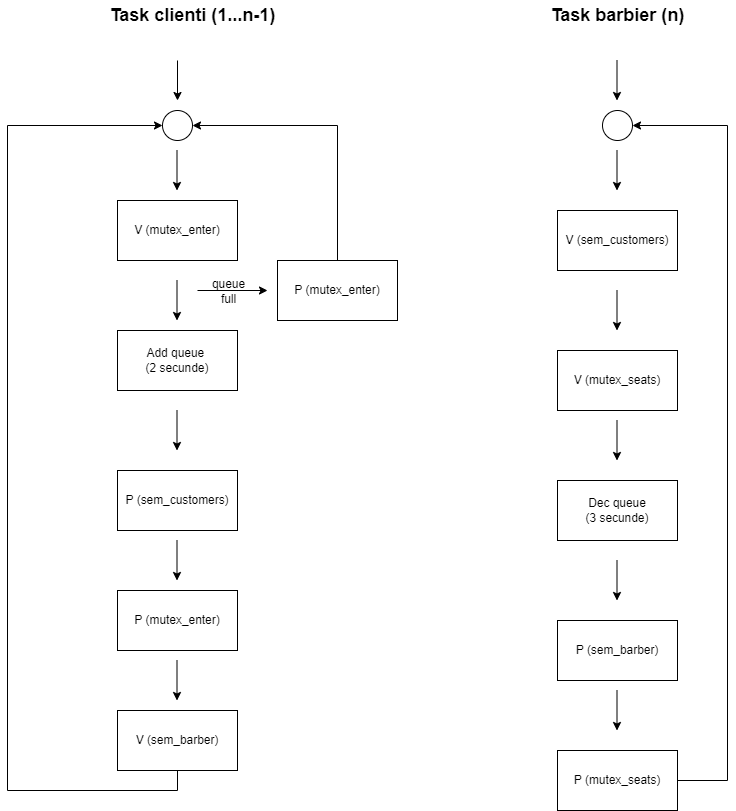
\includegraphics[width=12cm]{./images/Organigrama.png}
\caption{\label{fig:taskuri}Solu\c{t}ie implementare - organigrame taskuri}
\end{figure} 

Pentru crearea organigramelor, se poate folosi aplica\c{t}ia \textbf{Cmap}: \texttt{https://cmap.ihmc.us/}


\section{Implementarea solu\c{t}iei}

\^{I}n aceast\u{a} sec\c{t}iune se va prezenta codul aplica\c{t}iei. 

\paragraph{Se va comenta codul pentru a explica modul de lucru.}

\subsection*{Codul aplica\c{t}iei \^{i}n document}

\medskip
\medskip

\noindent
{\it \textbf{Task customers}:}
{\small
\begin{verbatim}
    while (!gata)
    {
        gettimeofday(&endCustomer, NULL);
        if(endCustomer.tv_sec - startCustomer.tv_sec >= timeCustomer) {
            pthread_mutex_lock(&mutex_enter);
            if ( !isFull(argum.Queue) && !gata) {
                printf("Ding! Ding! Clientul %s a intrat in sala. - %d\n", argum.nume, argum.ID);
                push(argum.Queue, argum.ID);
                sleep(2);
                sem_post(&sem_customers);
                pthread_mutex_unlock(&mutex_enter);
                sem_wait(&sem_barber);
            } else if(!gata){
                printf("Sala este plina, clientul %s pleaca. - %d\n", argum.nume, argum.ID);
                sleep(2);
                pthread_mutex_unlock(&mutex_enter);
            }
            else {
                pthread_mutex_unlock(&mutex_enter);
            }
            
            startCustomer = endCustomer;
            timeCustomer = rand() % 4;
        }  
    }
\end{verbatim}

Dacă bărbierul încă lucrează, se memorează momentul la care intră clientul în sală, acesta blocând mutex\_enter. În cazul în care mai este loc în coadă, clientul se așează la rând incrementând sem\_customers și deblocând mutex\_enter. În caul în care bărbierul este liber, sem\_barber se decrementează. Dacă sala este plină și programul de lucru încă nu s-a terminat, clientul pleacă și se deblochează mutex\_enter. Dacă programul s-a terminat, clientul nu mai intră în sală și se deblochează mutex\_enter. La final se resetează timpul după care intră următorul client (între 0 și 3 secunde).
\paragraph{}

{\large\it \textbf{Task barber}:}
{\small
\begin{verbatim}
   while (1)
    {
        sem_wait(&sem_customers);
        pthread_mutex_lock(&mutex_seats);
        sleep(3);
        printf("Barbierul a tuns un client - %d.\n", pop(argum.Queue));
       
        sem_post(&sem_barber);  
        pthread_mutex_unlock(&mutex_seats);
        gettimeofday(&end, NULL);
        if(end.tv_sec - start.tv_sec >= 20 && !gata) {
            gata = 1;
            printf("Programul de lucru s-a terminat, nu mai primim clienti!\n");
        }
        if(gata && isEmpty(argum.Queue)) {
            printf("Salonul s-a inchis, o zi buna!\n");
            break;
        }
    }
\end{verbatim}

Se verifică existența clienților în coadă și se decrementează sem\_customers. După aceea se blochează mutex\_seats (se așează un client pe scaunul bărbierului decrementându-se coada). Se incrementează sem\_barber după ce a terminat de tuns clientul și se deblochează mutex\_seats. Următoarele linii se referă la programul bărbierului, astfel că după un timp dat, 20 de secunde în cazul nostru, bărbierul nu mai acceptă clienți în coadă, terminând de tuns persoanele care așteaptă deja.

\paragraph{}

{\large\it \textbf{Funcții thread-uri}:}
{\small
\begin{verbatim}
   //Creearea threadurilor customers
    for (int i = 0; i < NUM_THREAD; i++) {
        if( pthread_create(&threads[i], NULL, customer, (void *)&arguments[i]) != 0 ) {
            perror("Pthread create customers.");
            return EXIT_FAILURE;
        }
    }

    //Creearea threadului barber
    if( pthread_create(&threads[NUM_THREAD], NULL, barber, (void *)&arguments[NUM_THREAD]) != 0 ) {
        perror("Pthread create barber.");
        return EXIT_FAILURE;
    }

    //Unirea threadurilor
    for (int i = 0; i <= NUM_THREAD; i++) {
        if( pthread_join(threads[i], NULL) != 0 ) {
            perror("Pthread join.");
            return EXIT_FAILURE;
        } 
    }

    pthread_mutex_destroy(&mutex_seats);
    sem_destroy(&sem_customers);
    sem_destroy(&sem_barber);
\end{verbatim}

}




\section{Testarea aplica\c{t}iei si validarea solu\c{t}iei propuse}

Aceast\u{a} sec\c{t}iune include comentarii despre modul \^{i}n care se execut\u{a} programul. Se ob\c{t}ine ceea ce s-a specificat la pasul 1, \^{i}n cerin\c{t}e?

Programul rulează conform descrierii din cadrul pasului 1, astfel obținându-se gestionarea și sincronizarea thread-urilor pentru îndeplinirea cerinței.

\paragraph{}

\begin{figure} [!htb]
\centering
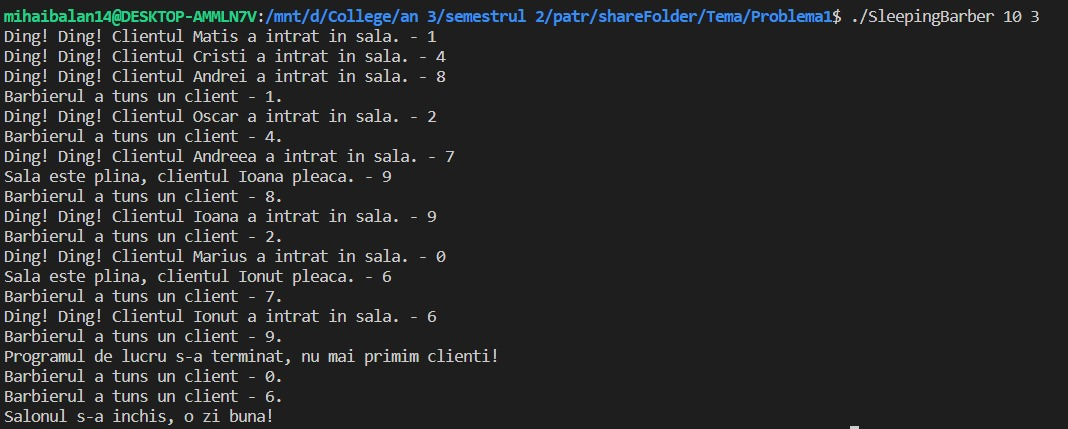
\includegraphics[width=12cm]{./images/Rezultat.jpeg}
\caption{\label{fig:taskuri}Rezultat execuție aplicație - 10 thread-uri și 3 locuri în coadă}
\end{figure} 


\end{document}
